\chapter{Rayonnement thermique}\label{ch:b2:thermal-radiation}

Tout ce qui est chaud rayonne. Une main, un mur, un verre d'eau à température
ambiante rayonnent invisiblement, à des longueurs d'onde voisines de \qty{10}{\micro m}, quelques
centaines de watts par mètre carré~; chauffez un tisonnier et à
\qty{600}{\celsius} il rougeoie sourdement, à \qty{1000}{\celsius} il est orange, à
\qty{2500}{\celsius} --- le filament d'une ampoule --- blanc~; la
surface du Soleil à \qty{5800}{K} rayonne d'un blanc jaune, soixante mégawatts par
mètre carré, et cette lumière, après huit minutes de voyage, est ce qui
maintient la Terre à une température où l'eau est liquide. Le rayonnement est
le troisième mode de transfert de chaleur et le seul qui traverse le vide~;
c'est aussi le lieu où la physique classique a échoué et où Planck,
en 1900, a dû introduire le quantum. Ce chapitre énonce la loi qu'il a
trouvée, en tire les deux résultats dont on se sert constamment ---
le déplacement de Wien et la loi de Stefan--Boltzmann --- et les applique
aux échanges entre corps, au Soleil et à la Terre, et au
modèle à une couche de l'\omterm{prop:b2:thermal-radiation:greenhouse}{effet de serre} qui fixe notre climat.

\begin{omfigure}
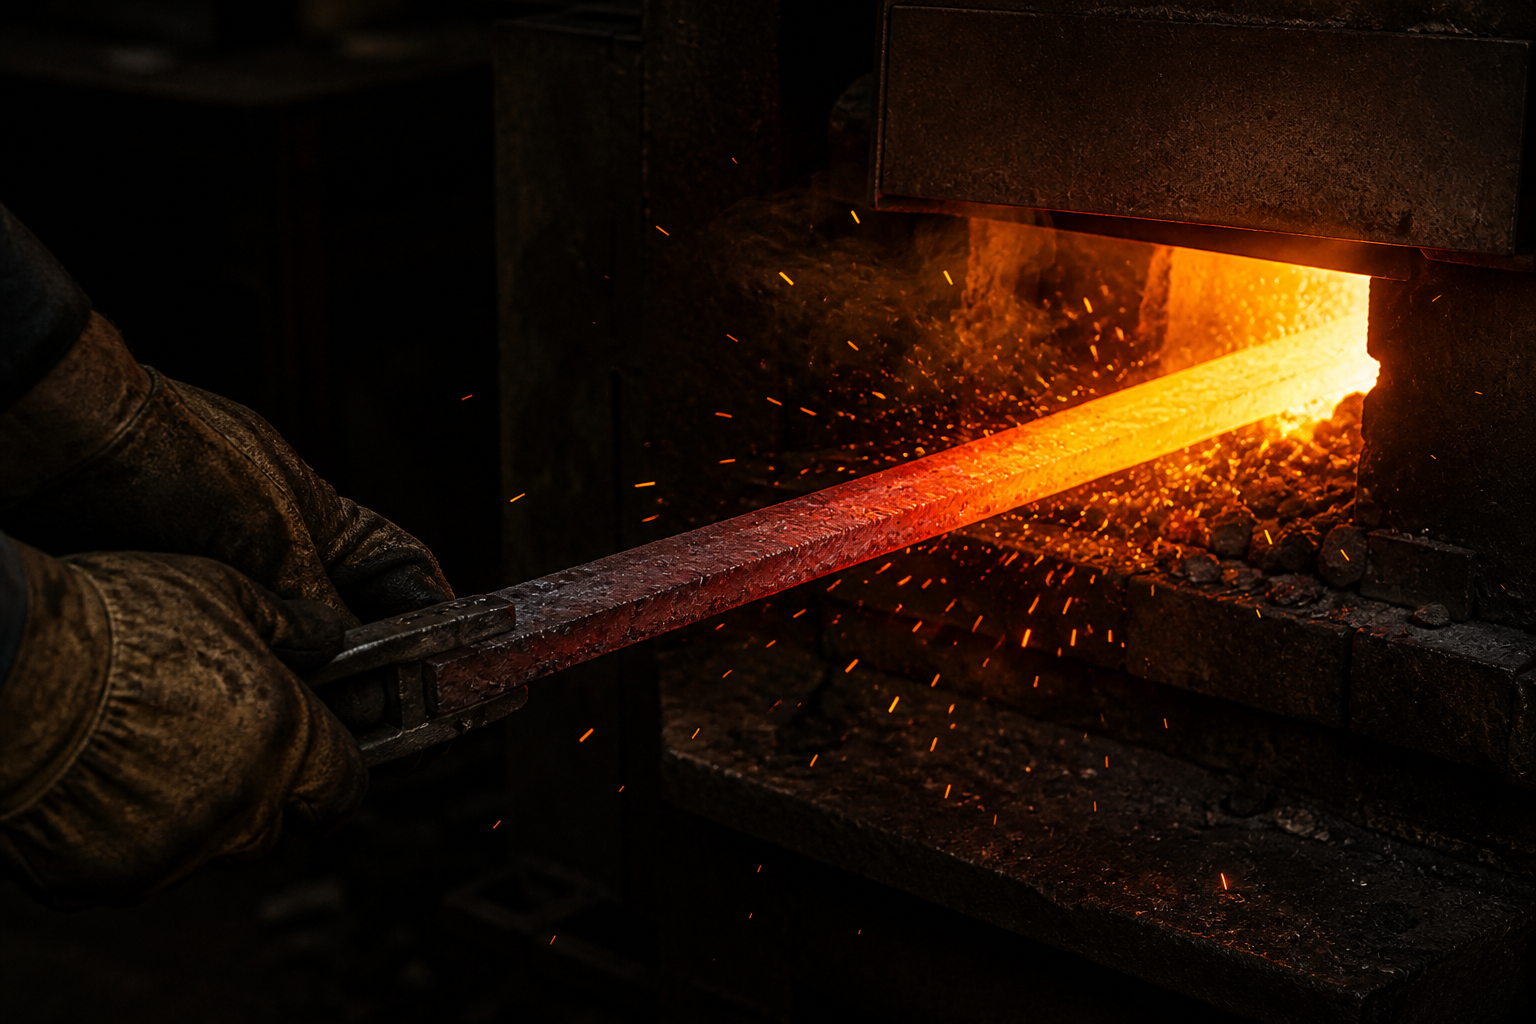
\includegraphics[width=0.58\linewidth]{images/book4/ai/b4-26-glowing-steel-forge.png}

{\small L'acier à la forge~: la couleur de l'incandescence --- rouge sombre, orange,
jaune, blanc --- est un thermomètre, parce que le spectre du \omterm{def:b2:thermal-radiation:blackbody}{rayonnement
thermique} ne dépend que de la température.}
\end{omfigure}

\section{Rayonnement thermique et corps noir}

\begin{definition}[Rayonnement thermique, absorptivité, corps noir]\label{def:b2:thermal-radiation:blackbody}
Tout corps à la température $T$ émet un rayonnement électromagnétique dû à
l'agitation thermique de ses charges~: son \emph{rayonnement
thermique}\index{rayonnement thermique}. Sa surface reçoit aussi du
rayonnement de son entourage et en absorbe une fraction $\alpha$
(l'\emph{absorptivité}, entre $0$ et $1$, dépendant en général de
la longueur d'onde), réfléchissant ou transmettant le reste. Un \emph{corps
noir}\index{corps noir} absorbe tout ($\alpha = 1$ à toute
longueur d'onde). Un petit trou dans la paroi d'une cavité fermée est le
corps noir pratique~: le rayonnement qui y entre est absorbé par les parois
avant d'avoir pu retrouver la sortie.
\end{definition}

\begin{proposition}[Rayonnement d'équilibre et loi de Kirchhoff]\label{prop:b2:thermal-radiation:kirchhoff}
À l'intérieur d'une cavité fermée dont les parois sont à $T$, le rayonnement est en
équilibre avec les parois et est \emph{universel}~: isotrope,
non polarisé, de densité spectrale d'énergie $u_\nu(T)$ (énergie par unité de
volume et de fréquence) qui ne dépend que de $T$ et de $\nu$, non du
matériau ni de la forme de la cavité. Le rayonnement qui sort d'un petit trou dans
une telle cavité est le \emph{rayonnement du \omterm{def:b2:thermal-radiation:blackbody}{corps noir}} à $T$. Une surface qui
absorbe la fraction $\alpha_\nu$ du rayonnement qu'elle reçoit à la
fréquence $\nu$ émet, à cette fréquence, la fraction
$\varepsilon_\nu = \alpha_\nu$ de ce qu'émettrait un \omterm{def:b2:thermal-radiation:blackbody}{corps noir} à la même
température (son \emph{émissivité}\index{émissivité})~:
\emph{les bons absorbeurs sont de bons émetteurs}.
\end{proposition}

\begin{proof}
Universalité~: reliez deux cavités à la même $T$ par un trou muni d'un
filtre laissant passer une fréquence~; si les densités différaient, l'énergie
s'écoulerait de l'une à l'autre à températures égales, en violation du second
principe. Kirchhoff~: placez la surface dans la cavité à sa propre $T$~; à
l'équilibre elle doit émettre à chaque fréquence exactement ce qu'elle absorbe,
$\varepsilon_\nu u_\nu = \alpha_\nu u_\nu$.
\end{proof}

\section{La loi de Planck}

\begin{theorem}[Loi de Planck]\label{thm:b2:thermal-radiation:planck}
La densité spectrale d'énergie du rayonnement du \omterm{def:b2:thermal-radiation:blackbody}{corps noir} à la température
$T$ vaut
\[
u_\nu(T) = \frac{8\pi h\nu^3}{c^3}\,\frac{1}{\eu^{h\nu/k_BT} - 1},
\]
et la puissance rayonnée par une surface noire par unité d'aire et par unité
de longueur d'onde (son \emph{exitance spectrale}\index{exitance spectrale}) vaut
\[
M_\lambda(T) = \frac{2\pi hc^2}{\lambda^5}\,\frac{1}{\eu^{hc/\lambda k_BT} - 1}.
\]
Deux limites~: pour $h\nu \ll k_BT$, $u_\nu \approx 8\pi\nu^2 k_BT/c^3$
(Rayleigh--Jeans~: chaque mode de la cavité porte l'énergie classique
$k_BT$ --- une loi dont l'intégrale diverge, la «~catastrophe
ultraviolette~»)~; pour $h\nu \gg k_BT$, $u_\nu \approx (8\pi h\nu^3/c^3)
\eu^{-h\nu/k_BT}$ (Wien~: le facteur de Boltzmann d'un photon d'énergie
$h\nu$, \cref{ch:b2:boltzmann-factor}).
\end{theorem}

\begin{proof}
Admis~: le dénombrement des modes de la cavité ($8\pi\nu^2/c^3$ par unité
de volume et de fréquence, deux polarisations) appartient au volume de troisième année,
et l'énergie moyenne d'un mode, $h\nu/(\eu^{h\nu/k_BT} - 1)$ au lieu du
$k_BT$ classique, est l'hypothèse quantique~: l'énergie est échangée avec
le mode par quanta $h\nu$, de sorte que les modes à $h\nu \gg k_BT$ sont
gelés. La relation $M_\lambda\,\dd\lambda = (c/4)\,u_\nu\,\dd\nu$ est le
facteur géométrique calculé dans le \cref{thm:b2:thermal-radiation:stefan}.
\end{proof}

\begin{omfigure}
\begin{tikzpicture}
  \begin{axis}[omaxis, width=9.2cm, height=5.2cm, xmin=0, xmax=3.1, ymin=0, ymax=1.12,
    xlabel={$\lambda$ (\unit{\micro m})}, ylabel={$M_\lambda$ (u.a.)}, xtick={0.5,1,1.5,2,2.5,3}, ytick=\empty, clip=false,
    legend style={font=\scriptsize, at={(0.97,0.95)}, anchor=north east, draw=none, fill=none}]
    \fill[yellow!40, opacity=0.6] (axis cs:0.4,0) rectangle (axis cs:0.7,1.08);
    \addplot[omDef, thick, domain=0.2:3.1, samples=160] {9.25*x^(-5)/(exp(14388/(x*5000))-1)};
    \addlegendentry{\qty{5000}{K}}
    \addplot[omThm, thick, domain=0.25:3.1, samples=160] {9.25*x^(-5)/(exp(14388/(x*4500))-1)};
    \addlegendentry{\qty{4500}{K}}
    \addplot[omExo, thick, domain=0.3:3.1, samples=160] {9.25*x^(-5)/(exp(14388/(x*4000))-1)};
    \addlegendentry{\qty{4000}{K}}
    \node[font=\scriptsize, anchor=south] at (axis cs:0.55,1.08) {visible};
  \end{axis}
\end{tikzpicture}

{\small Le spectre de Planck à trois températures~: le maximum se déplace vers les
courtes longueurs d'onde en $1/T$ (Wien) et l'aire croît en $T^4$
(Stefan). Seule la courbe la plus chaude met une part notable de sa puissance dans la bande
visible.}
\end{omfigure}

\begin{omfigure}
\begin{tikzpicture}
  \begin{axis}[omaxis, width=8.6cm, height=4.8cm, xmin=0, xmax=10.9, ymin=0, ymax=2.2,
    xlabel={$x = h\nu/k_BT$}, ylabel={$x^3/(\eu^x - 1)$}, xtick={2,4,6,8,10}, ytick={1,2}, clip=false,
    legend style={font=\scriptsize, at={(0.97,0.95)}, anchor=north east, draw=none, fill=none}]
    \addplot[omDef, thick, domain=0.05:10, samples=160] {x^3/(exp(x)-1)};
    \addlegendentry{Planck}
    \addplot[omExo, thick, dashed, domain=0.05:1.45, samples=60] {x^2};
    \addlegendentry{Rayleigh--Jeans $x^2$}
    \addplot[omThm, thick, dashed, domain=1.2:10, samples=100] {x^3*exp(-x)};
    \addlegendentry{Wien $x^3\eu^{-x}$}
  \end{axis}
\end{tikzpicture}

{\small La fonction de Planck et ses deux limites~: équipartition classique
à basse fréquence, coupure exponentielle de Boltzmann à haute fréquence~;
le maximum se situe en $x = 2.82$ (par unité de fréquence).}
\end{omfigure}

\begin{proposition}[Loi du déplacement de Wien]\label{prop:b2:thermal-radiation:wien}
L'\omterm{thm:b2:thermal-radiation:planck}{exitance spectrale} $M_\lambda$ est maximale en
\[
\lambda_{\max}\,T = \frac{hc}{4.965\,k_B} = \qty{2.90e-3}{m.K} .
\]
Un corps à \qty{300}{K} rayonne surtout vers \qty{10}{\micro m}~; le Soleil
(\qty{5800}{K}) vers \qty{0.5}{\micro m}, dans le vert, là où l'œil est le
plus sensible --- ce n'est pas un hasard.
\end{proposition}

\begin{proof}
Avec $x = hc/\lambda k_BT$, $M_\lambda \propto x^5/(\eu^x - 1)$~; $\dd/\dd x = 0$
donne $5(\eu^x - 1) = x\eu^x$, c'est-à-dire $x = 5(1 - \eu^{-x})$, dont la racine
non nulle vaut $x = 4.965$.
\end{proof}

\begin{theorem}[Loi de Stefan--Boltzmann]\label{thm:b2:thermal-radiation:stefan}
Une surface noire à $T$ rayonne, par unité d'aire, la puissance totale
\[
M = \int_0^\infty M_\lambda\,\dd\lambda = \sigma T^4, \qquad
\sigma = \frac{2\pi^5k_B^4}{15h^3c^2} = \qty{5.67e-8}{W/m^2/K^4} ;
\]
la densité d'énergie du rayonnement d'équilibre vaut $u = (4\sigma/c)T^4$
et sa pression $P = u/3$. Une surface grise d'\omterm{prop:b2:thermal-radiation:kirchhoff}{émissivité} $\varepsilon$
rayonne $\varepsilon\sigma T^4$.
\end{theorem}

\begin{proof}
Intégrons la densité de Planck~: $u = \int u_\nu\,\dd\nu = (8\pi h/c^3)(k_BT/h)^4
\int_0^\infty x^3\,\dd x/(\eu^x - 1)$ et l'intégrale vaut $\pi^4/15$
(admis de l'analyse)~: $u = (8\pi^5k_B^4/15h^3c^3)\,T^4$. La puissance
qui sort d'un trou d'aire unité dans la paroi de la cavité vaut $cu/4$~: le
rayonnement est isotrope, les photons se dirigeant vers le trou dans
l'angle solide $\dd\Omega$ sous l'angle $\theta$ à sa normale portent le
flux $c\,u\,(\dd\Omega/4\pi)\cos\theta$, et $\int\cos\theta\,\dd\Omega/4\pi$
sur l'hémisphère sortant vaut $1/4$. D'où $M = cu/4 = \sigma T^4$.
La pression, comme pour tout gaz isotrope de particules allant à $c$, vaut
$u/3$.
\end{proof}

\begin{example}[Ordres de grandeur]\label{ex:b2:thermal-radiation:orders}
À \qty{300}{K}~: $\sigma T^4 = \qty{460}{W/m^2}$ --- une personne de
\qty{1.7}{m^2} rayonne \qty{800}{W}, mais en reçoit presque autant des
murs à \qty{293}{K}~; la perte nette, $\sigma A(T^4 - T_0^4) \approx
\qty{100}{W}$, est toute la production métabolique du corps, d'où le fait qu'on
a besoin de vêtements dans une pièce qui semble douce. La surface du Soleil~: $\sigma
(5800)^4 = \qty{6.4e7}{W/m^2}$, au total $3.9 \times 10^{26}\,\unit{W}$. Le
filament d'une ampoule à \qty{2800}{K}~: \qty{3.5e6}{W/m^2}, \qty{60}{W} pour un
demi-centimètre carré de tungstène. Le fond diffus cosmologique, \qty{2.7}{K}~:
maximum à \qty{1}{mm}, $\qty{3e-6}{W/m^2}$, et $400$ photons par centimètre
cube d'univers.
\end{example}

\section{Échanges radiatifs}

\begin{proposition}[Échange net et coefficient radiatif]\label{prop:b2:thermal-radiation:exchange}
Un petit corps gris (\omterm{prop:b2:thermal-radiation:kirchhoff}{émissivité} $\varepsilon$, aire $S$, température $T$)
dans un vaste entourage à $T_0$ perd la puissance nette
\[
P = \varepsilon\sigma S\,(T^4 - T_0^4)
\ \approx\ 4\varepsilon\sigma T_0^3\,S\,(T - T_0) = h_{\text{r}}S(T - T_0)
\quad\text{pour } |T - T_0| \ll T_0 ,
\]
où $h_{\text{r}} = 4\varepsilon\sigma T_0^3 \approx \qty{6}{W/m^2/K}$ à
température ambiante --- comparable à la convection naturelle~: dans une pièce, le
rayonnement emporte environ la moitié de la chaleur qui quitte un corps ou un radiateur.
Entre deux grandes plaques noires parallèles la densité de flux nette vaut
$\sigma(T_1^4 - T_2^4)$~; pour des plaques grises d'\omterm{prop:b2:thermal-radiation:kirchhoff}{émissivités} $\varepsilon_1$,
$\varepsilon_2$ elle vaut $\sigma(T_1^4 - T_2^4)/(1/\varepsilon_1 + 1/\varepsilon_2
- 1)$, et chaque mince \emph{écran radiatif} intercalé la divise
encore --- le principe du vase Dewar et de la feuille d'or sur les
satellites.
\end{proposition}

\begin{proof}
Le corps émet $\varepsilon\sigma T^4$ et absorbe la fraction $\alpha =
\varepsilon$ du rayonnement noir $\sigma T_0^4$ qui emplit l'enceinte
(Kirchhoff). Linéariser $T^4 - T_0^4 \approx 4T_0^3(T - T_0)$. Pour les
plaques grises, sommer les réflexions multiples (une série géométrique).
\end{proof}

\begin{example}[Gelée sous un ciel clair, et la caméra thermique]\label{ex:b2:thermal-radiation:frost}
Par nuit claire le ciel rayonne comme un corps à environ \qty{250}{K}
(la haute atmosphère sèche), tandis que l'air près du sol est à
\qty{278}{K}. Une feuille ou un toit de voiture ($\varepsilon = 0.95$) équilibre sa
perte radiative vers le ciel par la convection venue de l'air ($h =
\qty{5}{W/m^2/K}$)~: $\varepsilon\sigma(T^4 - 250^4) = h(278 - T)$ donne $T
\approx \qty{266}{K}$ --- de la gelée à \qty{-7}{\celsius} sur l'herbe alors que
le thermomètre indique $+5$. Un nuage (rayonnant à \qty{275}{K}) relève $T$
à \qty{277}{K}~: pas de gelée. Une caméra thermique mesure la luminance vers
\qty{10}{\micro m} et la convertit en température en supposant
$\varepsilon \approx 0.95$~; un métal poli ($\varepsilon = 0.1$) réfléchit
surtout la pièce et apparaît à la température de la pièce quelle que soit la
sienne --- d'où le ruban noir que les thermographes collent sur les pièces brillantes.
\end{example}

\section{Le Soleil, la Terre et la serre}

\begin{proposition}[Constante solaire et température effective]\label{prop:b2:thermal-radiation:earth}
Le Soleil (rayon $R_\odot$, température de surface $T_\odot$) délivre à la
distance $d$ la densité de flux $S = \sigma T_\odot^4 (R_\odot/d)^2 =
\qty{1361}{W/m^2}$ au-dessus de l'atmosphère terrestre (la \emph{constante
solaire}\index{constante solaire}). Une planète d'albédo $A$ (la fraction
réfléchie) absorbe $(1 - A)S\pi R^2$ et, en régime permanent, le rayonne
depuis toute sa surface $4\pi R^2$ comme un \omterm{def:b2:thermal-radiation:blackbody}{corps noir} à sa \emph{température
effective}\index{température effective}
\[
T_{\text{e}} = \Big(\frac{(1 - A)S}{4\sigma}\Big)^{1/4} = \qty{255}{K}
\quad\text{pour la Terre } (A = 0.30) .
\]
\end{proposition}

\begin{proof}
Conservation de l'énergie~: absorbé $= $ émis, la section $\pi R^2$
pour le faisceau intercepté, la sphère entière pour l'émission (jour et
nuit, étalés par la rotation et la circulation).
\end{proof}

\begin{omfigure}
\begin{tikzpicture}[scale=0.95, >=stealth]
  % ground
  \fill[omExo!15] (0,0) rectangle (8,0.6);
  \draw[thick] (0,0.6) -- (8,0.6);
  \node[font=\scriptsize] at (4,0.3) {surface $T_{\text{s}}$};
  % atmosphere layer
  \fill[omDef!12] (0,2.6) rectangle (8,3.0);
  \draw (0,2.6) -- (8,2.6); \draw (0,3.0) -- (8,3.0);
  \node[font=\scriptsize] at (4.3,2.8) {atmosphère $T_{\text{a}}$};
  % solar in
  \draw[->, yellow!60!orange, very thick] (1.2,4.3) -- (1.2,0.7);
  \node[font=\scriptsize, yellow!50!orange, left] at (1.1,3.8) {$(1 - A)S/4$};
  % surface up
  \draw[->, omThm, very thick] (3.2,0.7) -- (3.2,2.5);
  \node[font=\scriptsize, omThm, right] at (3.25,1.6) {$\sigma T_{\text{s}}^4$};
  % atm up & down
  \draw[->, omDef, very thick] (5.4,3.1) -- (5.4,4.3);
  \node[font=\scriptsize, omDef, right] at (5.45,3.8) {$\sigma T_{\text{a}}^4$};
  \draw[->, omDef, very thick] (6.8,2.5) -- (6.8,0.7);
  \node[font=\scriptsize, omDef, right] at (6.85,1.6) {$\sigma T_{\text{a}}^4$};
  \node[font=\scriptsize] at (4,4.6) {espace};
\end{tikzpicture}

{\small La serre à une couche~: la lumière du Soleil traverse l'atmosphère et
réchauffe le sol~; l'infrarouge du sol est absorbé par la couche, qui
rayonne moitié vers le haut et moitié vers le bas --- la surface doit alors rayonner deux fois
ce qu'elle reçoit du Soleil.}
\end{omfigure}

\begin{proposition}[Modèle de serre à une couche]\label{prop:b2:thermal-radiation:greenhouse}
Entourons la planète d'une mince couche d'atmosphère transparente
à la lumière du Soleil mais absorbant tout l'infrarouge émis par la surface, et
rayonnant comme un \omterm{def:b2:thermal-radiation:blackbody}{corps noir} à $T_{\text{a}}$ vers le haut comme vers le bas. En régime
permanent,
\[
T_{\text{a}} = T_{\text{e}}, \qquad
T_{\text{s}} = 2^{1/4}\,T_{\text{e}} = \qty{303}{K} .
\]
Si la couche n'absorbe que la fraction $\varepsilon$ de l'infrarouge,
$T_{\text{s}}^4 = T_{\text{e}}^4/(1 - \varepsilon/2)$~; les \qty{288}{K}
observés correspondent à $\varepsilon \approx 0.78$. La surface est
plus chaude que la \omterm{prop:b2:thermal-radiation:earth}{température effective} parce qu'elle reçoit, en plus
du Soleil, l'infrarouge que l'atmosphère lui renvoie ---
l'\emph{effet de serre}\index{effet de serre}, \qty{33}{K} sur Terre,
sans lequel les océans seraient gelés.
\end{proposition}

\begin{proof}
Bilan de la couche~: elle absorbe $\sigma T_{\text{s}}^4$, émet $2\sigma
T_{\text{a}}^4$. Bilan de la planète vue de l'espace~: elle émet $\sigma
T_{\text{a}}^4 = (1 - A)S/4 = \sigma T_{\text{e}}^4$. Bilan de la
surface~: elle reçoit $(1 - A)S/4 + \sigma T_{\text{a}}^4 = 2\sigma T_{\text{e}}^4$,
elle émet $\sigma T_{\text{s}}^4$. Pour la couche partielle, remplacer
l'infrarouge absorbé et émis par $\varepsilon\sigma T_{\text{s}}^4$ et
$\varepsilon\sigma T_{\text{a}}^4$ et laisser la fraction $1 - \varepsilon$
du rayonnement de surface s'échapper directement.
\end{proof}

\begin{omfigure}
\begin{tikzpicture}
  \begin{axis}[width=9.6cm, height=5cm, xmode=log, xmin=0.1, xmax=100, ymin=0, ymax=1.15,
    axis x line=bottom, axis y line=left, xlabel={$\lambda$ (\unit{\micro m})}, ylabel={$M_\lambda$ (normalisé)},
    xlabel style={at={(axis description cs:0.5,-0.12)}, anchor=north},
    xtick={0.1,1,10,100}, xticklabels={$0.1$,$1$,$10$,$100$}, ytick=\empty, clip=false,
    legend style={font=\scriptsize, at={(0.02,0.97)}, anchor=north west, draw=none, fill=none}]
    \fill[omDef!10] (axis cs:5,0) rectangle (axis cs:8,1.0);
    \fill[omDef!10] (axis cs:14,0) rectangle (axis cs:17,1.0);
    \fill[gray!10] (axis cs:2.6,0) rectangle (axis cs:2.9,1.0);
    \addplot[yellow!60!orange, thick, domain=0.1:8, samples=200] {4.4*x^(-5)/(exp(14388/(x*5800))-1)};
    \addlegendentry{Soleil, \qty{5800}{K}}
    \addplot[omExo, thick, domain=2.5:100, samples=200] {1.41e7*x^(-5)/(exp(14388/(x*288))-1)};
    \addlegendentry{Terre, \qty{288}{K}}
    \node[font=\tiny, omDef, anchor=south] at (axis cs:6.3,1.0) {H$_2$O};
    \node[font=\tiny, omDef, anchor=south] at (axis cs:15.5,1.0) {CO$_2$};
    \node[font=\tiny, anchor=south] at (axis cs:10.5,0.2) {fenêtre};
  \end{axis}
\end{tikzpicture}

{\small Les spectres du Soleil et de la Terre (chacun normalisé à son
maximum) se recouvrent à peine~: l'atmosphère peut être transparente à l'un et
opaque à l'autre. En grisé~: les principales bandes d'absorption infrarouge de la
vapeur d'eau et du dioxyde de carbone~; entre elles la fenêtre \qty{8}{}--\qty{13}{\micro m}
par laquelle la surface rayonne directement vers l'espace.}
\end{omfigure}

\begin{remark}[Pourquoi la serre est sélective]\label{rem:b2:thermal-radiation:selective}
La lumière solaire culmine à \qty{0.5}{\micro m}, le rayonnement de la Terre à
\qty{10}{\micro m}~: les deux spectres ne se recouvrent guère, si bien qu'un gaz peut être
transparent au premier et absorbant pour le second. L'azote et l'oxygène
n'absorbent ni l'un ni l'autre~; la vapeur d'eau, le dioxyde de carbone, le méthane et l'ozone
ont des bandes de vibration dans l'infrarouge et sont les gaz à \omterm{prop:b2:thermal-radiation:greenhouse}{effet de serre}. La
fenêtre entre \qty{8}{} et \qty{13}{\micro m} est celle que la caméra thermique
regarde, celle à laquelle se rapportent les \qty{250}{K} du ciel nocturne, et celle qu'exploitent
les peintures à refroidissement radiatif. Le verre d'une vraie serre fait
de même (transparent à \qty{0.5}{\micro m}, opaque à \qty{10}{\micro m}),
mais surtout il bloque la convection --- le nom est un peu injuste.
\end{remark}

\begin{method}[Estimations de rayonnement]\label{meth:b2:thermal-radiation:method}
(1) $\lambda_{\max} = \qty{2900}{\micro m.K}/T$ dit où se situe le spectre~;
(2) $\varepsilon\sigma T^4$ par unité d'aire~; (3) échanges~: émis
moins absorbé, linéarisé en $h_{\text{r}} = 4\varepsilon\sigma T^3$ près de la
température ambiante~; (4) une planète~: $(1 - A)S/4 = \sigma T_{\text{e}}^4$, puis
les couches~; (5) comparer à la conduction et à la convection --- le rayonnement
l'emporte à haute température ($T^4$) et dans le vide~; (6) attention aux \omterm{prop:b2:thermal-radiation:kirchhoff}{émissivités}~:
métaux brillants \qty{0.05}{}, peintures, peau, eau, sol $\approx 0.9$--$0.98$
dans l'infrarouge quelle que soit leur couleur visible.
\end{method}

\section{Exercices}

\begin{exercise}[$\star$]\label{exo:b2:thermal-radiation:1}
$\lambda_{\max}$ et $\sigma T^4$ pour~: le Soleil (\qty{5800}{K}), un humain
(\qty{310}{K}), le filament d'une ampoule (\qty{2800}{K}), le fond diffus cosmologique
(\qty{2.73}{K}), l'azote liquide (\qty{77}{K}), un tisonnier chauffé au rouge
(\qty{900}{K}). Lesquels sont visibles~?
\end{exercise}

\begin{exercise}[$\star$]\label{exo:b2:thermal-radiation:2}
À partir de $T_\odot = \qty{5772}{K}$, $R_\odot = \qty{6.96e8}{m}$, $d = \qty{1.496e11}{m}$~:
la \omterm{prop:b2:thermal-radiation:earth}{constante solaire}, la luminosité du Soleil, la puissance interceptée par la
Terre ($R = \qty{6.37e6}{m}$), et la même divisée entre $8 \times 10^9$
personnes. Comparer à la consommation mondiale de puissance (\qty{2e13}{W}).
\end{exercise}

\begin{exercise}[$\star$]\label{exo:b2:thermal-radiation:3}
Une personne~: peau à \qty{306}{K}, $\varepsilon = 0.98$, \qty{1.7}{m^2}, dans une
pièce à \qty{293}{K}. Puissance émise, puissance absorbée, perte nette~; le
coefficient radiatif $h_{\text{r}}$~; comparer aux \qty{100}{W} du
métabolisme et conclure sur les vêtements et sur une pièce à \qty{20}{\celsius}
aux murs froids.
\end{exercise}

\begin{exercise}[$\star$]\label{exo:b2:thermal-radiation:4}
Une ampoule de \qty{60}{W}~: filament de tungstène à \qty{2800}{K}, $\varepsilon = 0.35$.
Aire rayonnante~; longueur d'un fil de \qty{50}{\micro m} ayant cette aire~;
environ $8\%$ de la puissance est visible~: puissance lumineuse~; une LED donnant la
même lumière avec un rendement de $30\%$.
\end{exercise}

\begin{exercise}[$\star\star$]\label{exo:b2:thermal-radiation:5}
\emph{Les deux limites.} (a) Développer le $u_\nu$ de Planck pour $h\nu \ll k_BT$ et
identifier l'énergie par mode. (b) Montrer que la loi de Rayleigh--Jeans
donne une énergie totale infinie. (c) À \qty{300}{K}, la fréquence où
$h\nu = k_BT$~; en conclure que le \omterm{def:b2:thermal-radiation:blackbody}{rayonnement thermique} radio et micro-onde est
classique. (d) Dans la limite de Wien, interpréter $\eu^{-h\nu/k_BT}$.
\end{exercise}

\begin{exercise}[$\star\star$]\label{exo:b2:thermal-radiation:6}
\emph{Wien.} (a) Établir $x = 5(1 - \eu^{-x})$ et le résoudre numériquement
à trois chiffres. (b) Valeur de $\lambda_{\max}T$. (c) Montrer que $u_\nu$
est maximal en $h\nu = 2.82\,k_BT$, et que cela ne correspond pas à
$c/\lambda_{\max}$~: pourquoi~? (d) Température d'une étoile dont le spectre
culmine à \qty{290}{nm}~; sa couleur à l'œil.
\end{exercise}

\begin{exercise}[$\star\star$]\label{exo:b2:thermal-radiation:7}
\emph{Stefan.} (a) Mener l'intégration de la loi de Planck, sachant que
$\int_0^\infty x^3\dd x/(\eu^x - 1) = \pi^4/15$, et la valeur de $\sigma$.
(b) Justifier le facteur $c/4$ entre la densité et l'exitance. (c)
Sachant que $\int_0^\infty x^2\dd x/(\eu^x - 1) = 2.404$, le nombre de photons
par unité de volume à $T$, et l'énergie moyenne d'un photon en unités de $k_BT$.
(d) Photons par centimètre cube à \qty{300}{K} et à \qty{2.73}{K}.
\end{exercise}

\begin{exercise}[$\star\star$]\label{exo:b2:thermal-radiation:8}
\emph{Écrans.} Deux grandes plaques noires à $T_1$, $T_2$. (a) Flux net.
(b) On place entre elles une feuille noire mince~: sa température et le
flux nouveau. (c) $n$ feuilles. (d) Plaques grises d'\omterm{prop:b2:thermal-radiation:kirchhoff}{émissivité} $\varepsilon$~:
montrer que le flux vaut $\sigma(T_1^4 - T_2^4)/(2/\varepsilon - 1)$ et le calculer
pour des surfaces polies ($\varepsilon = 0.05$) à \qty{300}{K} et
\qty{77}{K} --- le vase Dewar.
\end{exercise}

\begin{exercise}[$\star\star$]\label{exo:b2:thermal-radiation:9}
\emph{Gelée nocturne.} Surface $\varepsilon = 0.95$, ciel à \qty{250}{K}, air à
\qty{278}{K} avec $h = \qty{5}{W/m^2/K}$. (a) Écrire le bilan et le résoudre
pour la température de surface. (b) Sous un nuage à \qty{275}{K}. (c) Pourquoi
le vent empêche-t-il la gelée~? (d) Pourquoi une voiture garée sous un arbre y
échappe-t-elle~?
\end{exercise}

\begin{exercise}[$\star\star\star$]\label{exo:b2:thermal-radiation:10}
\emph{Planètes.} (a) \omterm{prop:b2:thermal-radiation:earth}{Températures effectives} de Vénus ($S = \qty{2600}{W/m^2}$,
$A = 0.75$), de la Terre, de Mars ($S = \qty{590}{W/m^2}$, $A = 0.25$). (b) Leurs
températures de surface valent \qty{737}{K}, \qty{288}{K}, \qty{215}{K}~:
réchauffement de serre de chacune. (c) Dans le modèle à $n$ couches opaques,
montrer $T_{\text{s}}^4 = (n + 1)T_{\text{e}}^4$~; combien de couches pour Vénus~?
(d) La Lune~: $A = 0.12$, pas d'atmosphère, rotation lente --- température
du point subsolaire, et pourquoi la face nocturne tombe à \qty{100}{K}.
\end{exercise}

\begin{exercise}[$\star\star\star$]\label{exo:b2:thermal-radiation:11}
\emph{Sensibilité climatique sans \omterm{def:b2:feedback-oscillators:loop}{rétroactions}.} (a) Linéariser le
bilan planétaire~: un petit forçage supplémentaire $\Delta F$ (en \unit{W/m^2}) au
sommet de l'atmosphère élève la \omterm{prop:b2:thermal-radiation:earth}{température effective} de $\Delta T
= \Delta F/4\sigma T_{\text{e}}^3$. Calculer $4\sigma T_{\text{e}}^3$. (b)
Doubler le dioxyde de carbone est un forçage d'environ \qty{3.7}{W/m^2}~:
$\Delta T$ dans ce modèle. (c) La couche de mélange de l'océan (\qty{50}{m}
d'eau) emmagasine la chaleur~: constante de temps de la réponse. (d) Pourquoi les
\omterm{def:b2:feedback-oscillators:loop}{rétroactions} de la vapeur d'eau et de l'albédo de la glace rendent-elles la sensibilité réelle plus grande
que celle de (b)~?
\end{exercise}

\begin{exercise}[$\star\star\star$]\label{exo:b2:thermal-radiation:12}
\emph{Pyrométrie.} (a) Dans la limite de Wien, montrer que le rapport des
luminances à deux longueurs d'onde, $\lambda_1$ et $\lambda_2$, donne $T$
indépendamment d'une \omterm{prop:b2:thermal-radiation:kirchhoff}{émissivité} grise. (b) Une barre d'acier~: $M_{0.65}/M_{0.9}
= 0.10$~: température. (c) Une caméra thermique à \qty{10}{\micro m} suppose
$\varepsilon = 0.95$~; elle regarde de l'aluminium poli ($\varepsilon = 0.1$)
à \qty{350}{K} dans une pièce à \qty{293}{K}~: en régime linéarisé,
quelle température annonce-t-elle~? (d) Pourquoi une surface peinte à côté de
l'aluminium, à la même \qty{350}{K}, se lit-elle correctement~?
\end{exercise}

\begin{omfigure}
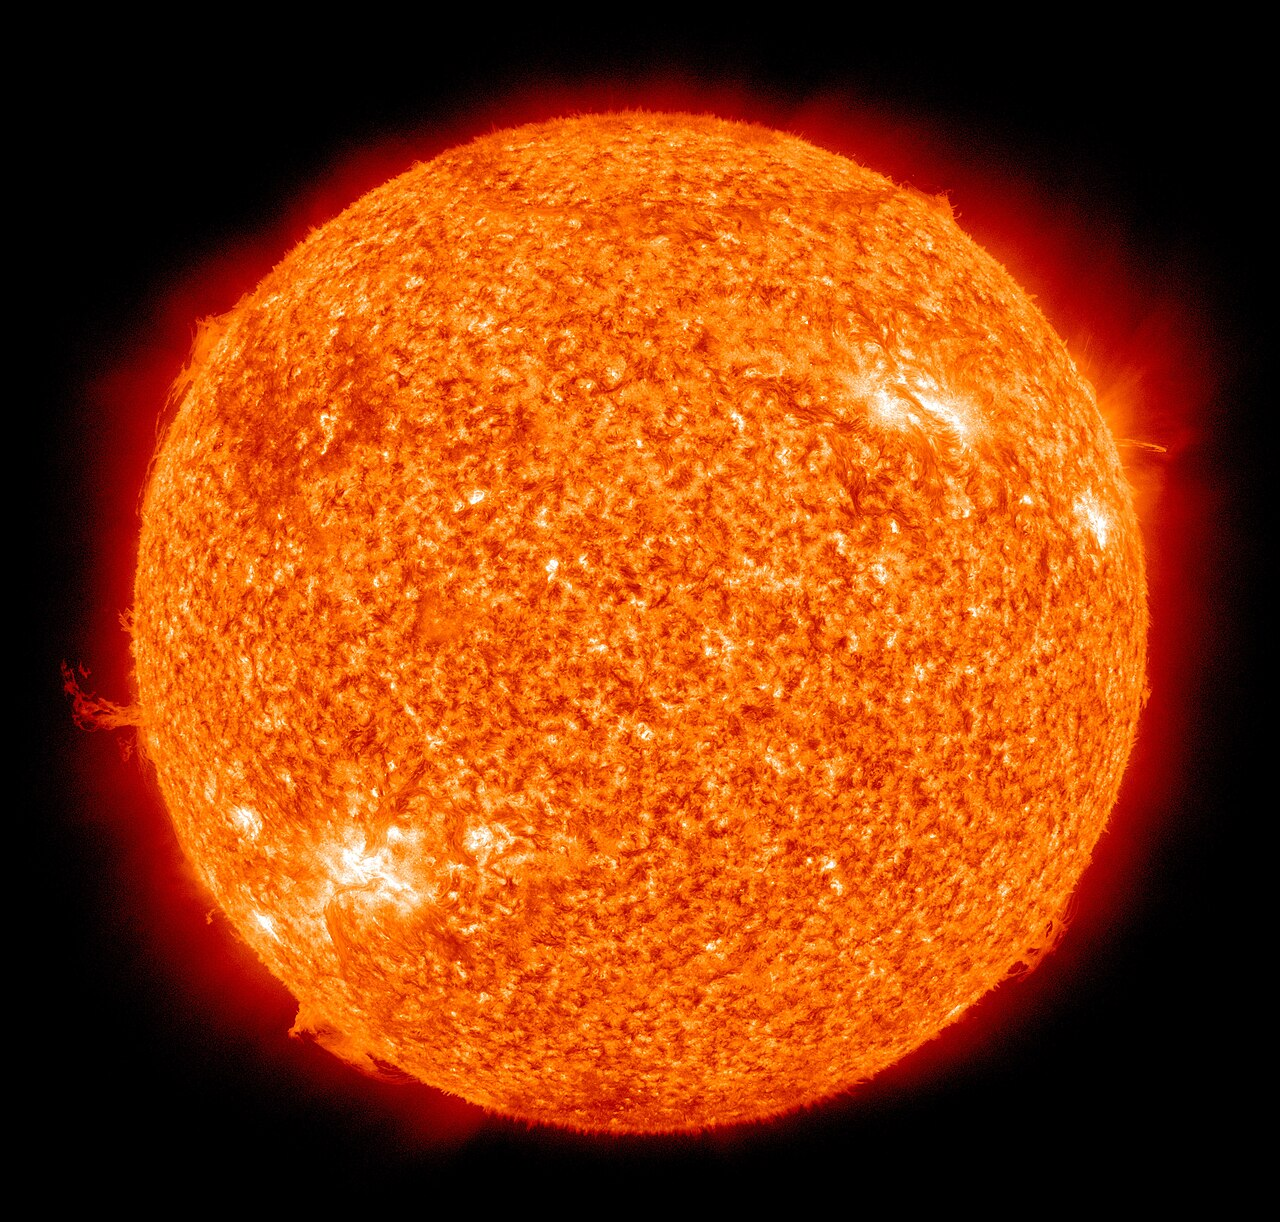
\includegraphics[width=0.4\linewidth]{images/book4/sun-sdo-aia.jpg}\hfill
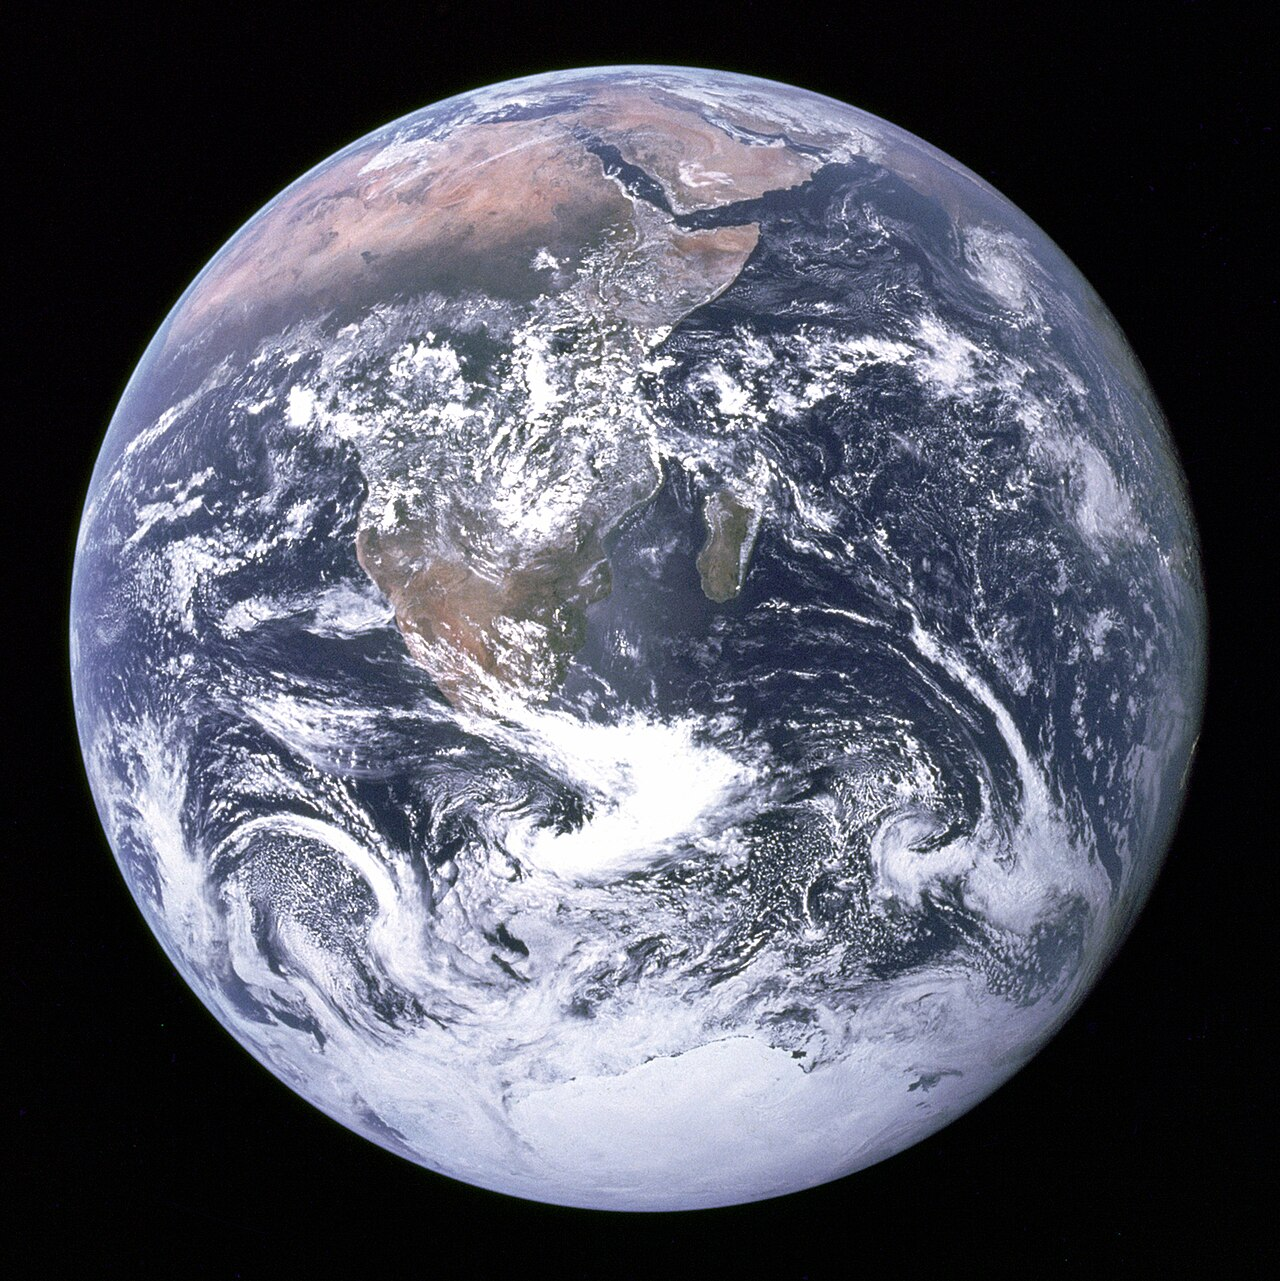
\includegraphics[width=0.4\linewidth]{images/book4/earth-apollo17.jpg}

{\small Les deux \omterm{def:b2:thermal-radiation:blackbody}{corps noirs} de ce chapitre~: le Soleil, à \qty{5800}{K}, vu par le Solar Dynamics Observatory dans l'ultraviolet extrême, et la Terre, à \qty{288}{K}, photographiée par l'équipage d'Apollo 17 --- maxima à \qty{0.5}{\micro m} et à \qty{10}{\micro m} (NASA).}
\end{omfigure}

\section{Problème~: le bilan énergétique de la Terre et l'ampoule à incandescence}

\begin{problem}[{Problème du week-end --- des corps noirs, du Soleil au
filament}]\label{pb:b2:thermal-radiation:1}
Données~: $\sigma = \qty{5.67e-8}{W/m^2/K^4}$, $\lambda_{\max}T = \qty{2.90e-3}{m.K}$,
$h = \qty{6.63e-34}{J.s}$, $k_B = \qty{1.38e-23}{J/K}$, $c = \qty{3.00e8}{m/s}$~;
Soleil~: $R_\odot = \qty{6.96e8}{m}$, $d = \qty{1.50e11}{m}$~; Terre~: $R =
\qty{6.37e6}{m}$, albédo $0.30$.

\textbf{Partie I --- Le Soleil comme \omterm{def:b2:thermal-radiation:blackbody}{corps noir}.}
\begin{enumerate}
  \item Le spectre solaire culmine à \qty{0.50}{\micro m}~: température
        de surface.
  \item Exitance de la surface et luminosité totale.
  \item \omterm{prop:b2:thermal-radiation:earth}{Constante solaire} à la Terre~; densité d'énergie et pression de
        la lumière solaire là-bas.
  \item Énergie moyenne d'un photon ($\approx 2.7\,k_BT$) et nombre de photons
        solaires par seconde et par mètre carré à la Terre.
  \item Le Soleil rayonne à ce rythme depuis $4.5 \times 10^9$ ans~:
        énergie émise~; comparer à $Mc^2$ pour $M = \qty{2e30}{kg}$.
\end{enumerate}

\textbf{Partie II --- La Terre sans atmosphère.}
\begin{enumerate}[resume]
  \item Puissance absorbée par la Terre~; \omterm{prop:b2:thermal-radiation:earth}{température effective}.
  \item Pourquoi le bilan divise-t-il par $4$~? Quelle serait la
        température au point subsolaire d'une Terre sans air et sans
        rotation ($A = 0.30$)~?
  \item La Lune ($A = 0.12$)~: température subsolaire~; et pourquoi sa face
        nocturne descend à \qty{100}{K} (penser à la chaleur emmagasinée dans le
        régolithe pendant les deux semaines de jour, \qty{1e6}{J/m^2/K} en effectif).
  \item Longueur d'onde du maximum d'émission de la Terre~; comparer à celle
        du Soleil.
  \item Si davantage de glace ou de nuages portait l'albédo à $0.35$, de combien
        la \omterm{prop:b2:thermal-radiation:earth}{température effective} baisserait-elle~?
\end{enumerate}

\textbf{Partie III --- La serre.}
\begin{enumerate}[resume]
  \item Écrire les trois bilans (espace, couche, surface) du
        modèle à une couche et obtenir $T_{\text{s}} = 2^{1/4}T_{\text{e}}$.
  \item Avec une couche absorbant la fraction $\varepsilon$ de
        l'infrarouge~: $T_{\text{s}}(\varepsilon)$~; la valeur de $\varepsilon$
        donnant \qty{288}{K}.
  \item Quels gaz absorbent, lesquels non, et dans quelle bande de longueurs
        d'onde~; qu'est-ce que la fenêtre atmosphérique~?
  \item L'infrarouge renvoyé au sol par l'atmosphère,
        en \unit{W/m^2}, dans le modèle à $\varepsilon = 0.78$~; comparer à
        la lumière solaire absorbée.
  \item Un forçage de \qty{3.7}{W/m^2} (dioxyde de carbone doublé)~:
        variation de température $\Delta T = \Delta F/4\sigma T_{\text{e}}^3$
        sans \omterm{def:b2:feedback-oscillators:loop}{rétroactions}.
  \item Capacité thermique d'une couche de mélange océanique de \qty{50}{m} par mètre
        carré et constante de temps de la réponse.
  \item Pourquoi les nuages refroidissent-ils (albédo) et réchauffent-ils (infrarouge) à la fois la
        surface~; quel effet l'emporte la nuit~?
\end{enumerate}

\textbf{Partie IV --- L'ampoule à incandescence.}
Une ampoule de \qty{60}{W} a un filament de tungstène à \qty{2800}{K},
$\varepsilon = 0.35$~; la fraction de la puissance d'un \omterm{def:b2:thermal-radiation:blackbody}{corps noir} qui tombe dans
le visible ($0.4$--\qty{0.7}{\micro m}) vaut $0.08$ à \qty{2800}{K} et $0.14$
à \qty{3200}{K}.
\begin{enumerate}[resume]
  \item Aire rayonnante du filament~; longueur d'un fil de \qty{50}{\micro m}
        qui l'a~; pourquoi est-il enroulé~?
  \item Longueur d'onde du maximum~; puissance visible~; rendement lumineux.
  \item Résistance du filament en fonctionnement sous \qty{230}{V}~;
        la résistivité du tungstène est environ dix fois plus faible à température
        ambiante~: courant à l'allumage, et une conséquence.
  \item À \qty{3200}{K}~: l'aire nécessaire pour les mêmes \qty{60}{W} et
        la puissance visible~; pourquoi ne pas faire fonctionner toute ampoule à \qty{3200}{K}
        (le taux d'évaporation du tungstène double à peu près tous les
        \qty{50}{K})~?
  \item Que fait le cycle halogène, et pourquoi permet-il un filament plus
        chaud~?
  \item Où passe le reste des \qty{60}{W}, et pourquoi le verre de
        l'ampoule atteint-il \qty{150}{\celsius}~?
  \item Temps de refroidissement du filament une fois éteint~: l'estimer à partir de
        sa masse (\qty{20}{mg}, $c = \qty{140}{J/kg/K}$) et de sa puissance
        rayonnée.
  \item Résumer~: ce que fixe la température d'un \omterm{def:b2:thermal-radiation:blackbody}{corps noir}, et ce que
        le filament, le Soleil et la Terre ont en commun.
\end{enumerate}
\end{problem}
